\chapter{Introduction}
\section{Motivation}
Many applications require a fast, structured data store. Correctly implementing
a custom solution in a general purpose programming language is a development cost.
Relational databases provide an attrative interface for describing the structure
and interfactions with a store, but come with performance caveats.
\\
\\ For example a common OLTP pattern is to use a database to store the current state of a service.
\begin{center}
    
\includegraphics[scale=1]{_drawio/introduction/images/slow_delta.pdf}
\end{center}
\vspace{-1cm}
\noindent For many such applications the following holds.
\begin{enumerate}
    \setlength\itemsep{0em}
    \item Persistence requirements are weak enough to allow for in-memory only storage (optionally durability by replication).
    \item Each instance of the application is the sole interactor with the data store.
    \item Invariants/Constraints about the data must be maintained by the store.
    \item The schema and parameterized queries used are known at compile time. \label{lab:known_queries_item}
\end{enumerate}
Another more common pattern is to use implement complex state of an application in a general purpose programming language.
\begin{center}
    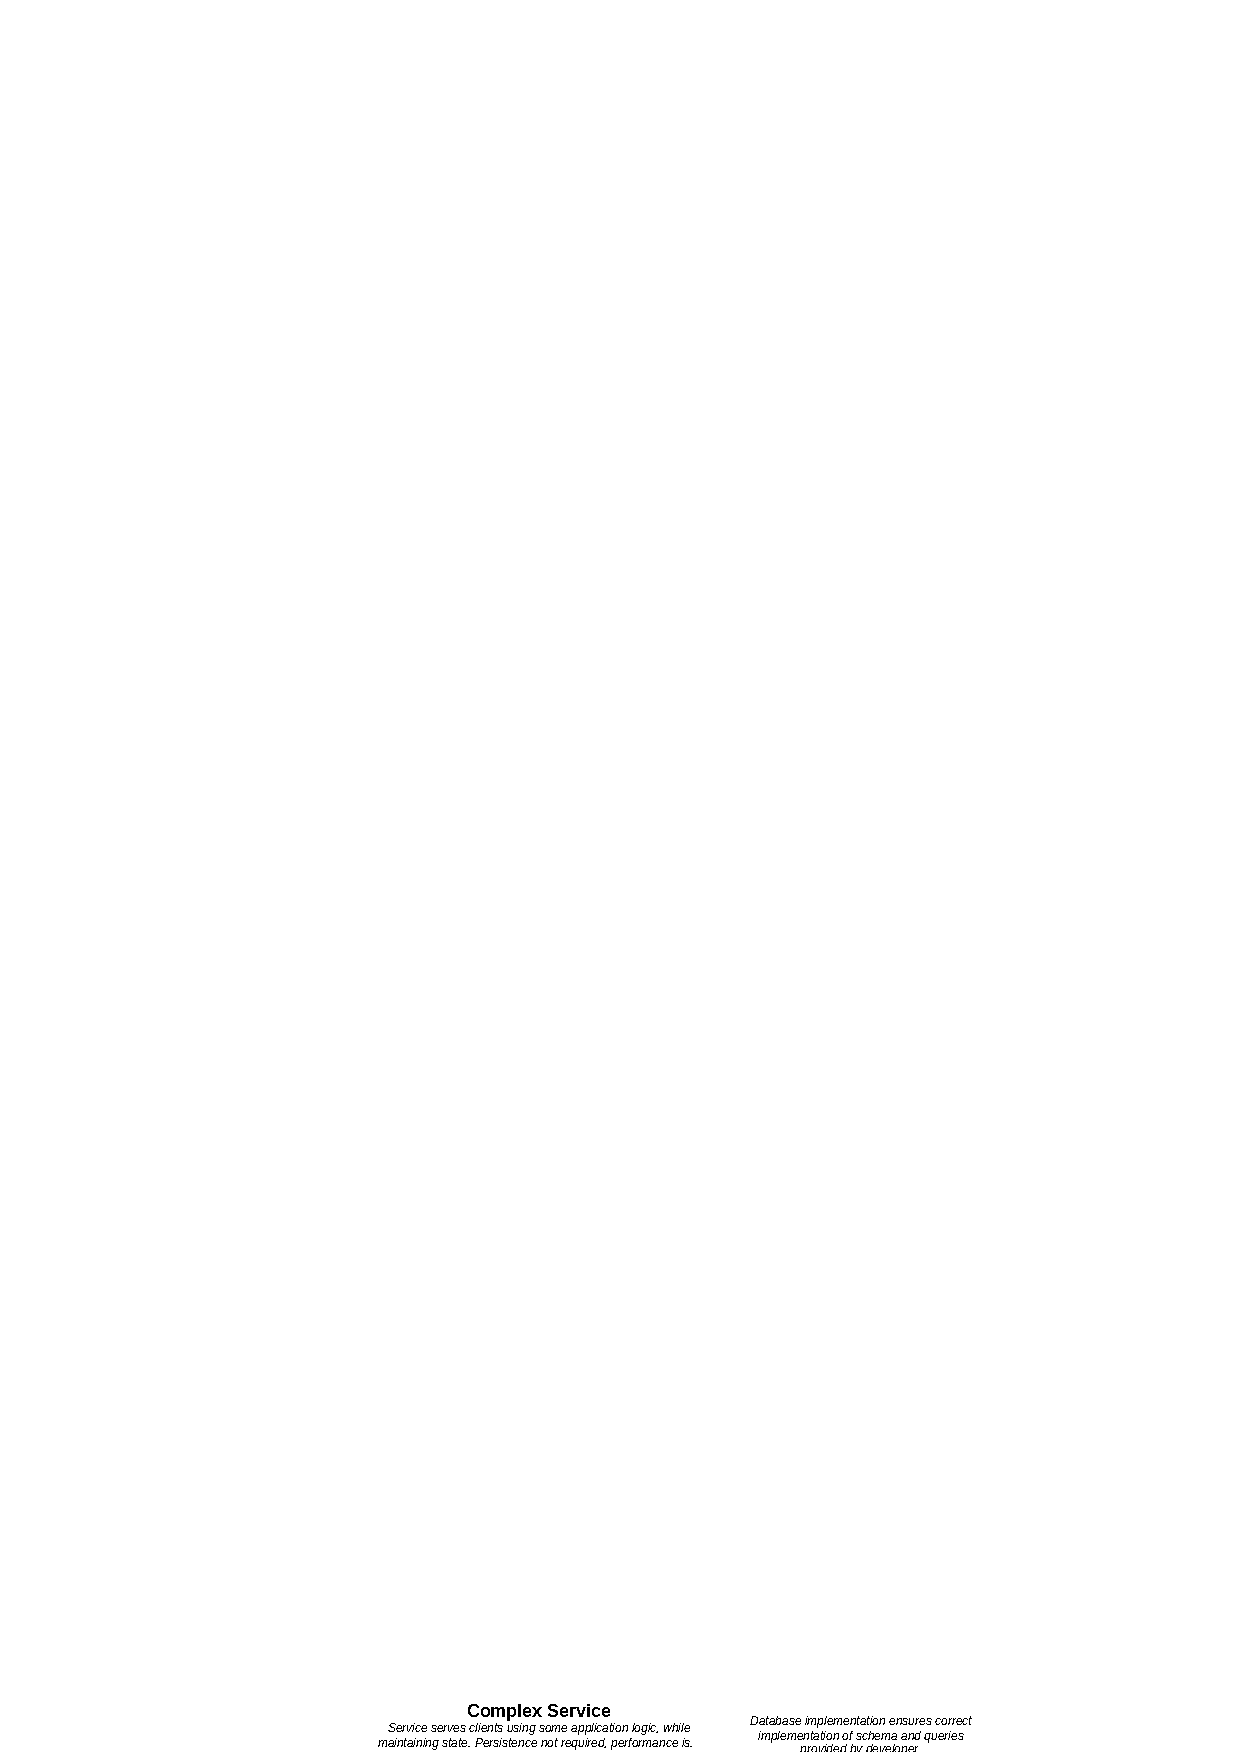
\includegraphics[scale=1]{_drawio/introduction/images/complex_service.pdf}
\end{center}
Much like the first pattern, a schema and set of queries including constraints are present, however the
burden is either on the programmer to implement, or on the performance of the application when using the
convenience of a query language \& database.
\\
\\ A spectrum of solutions exist to embed a store in an application, here generally placed according to the strength of abstraction provided.
\begin{center}
    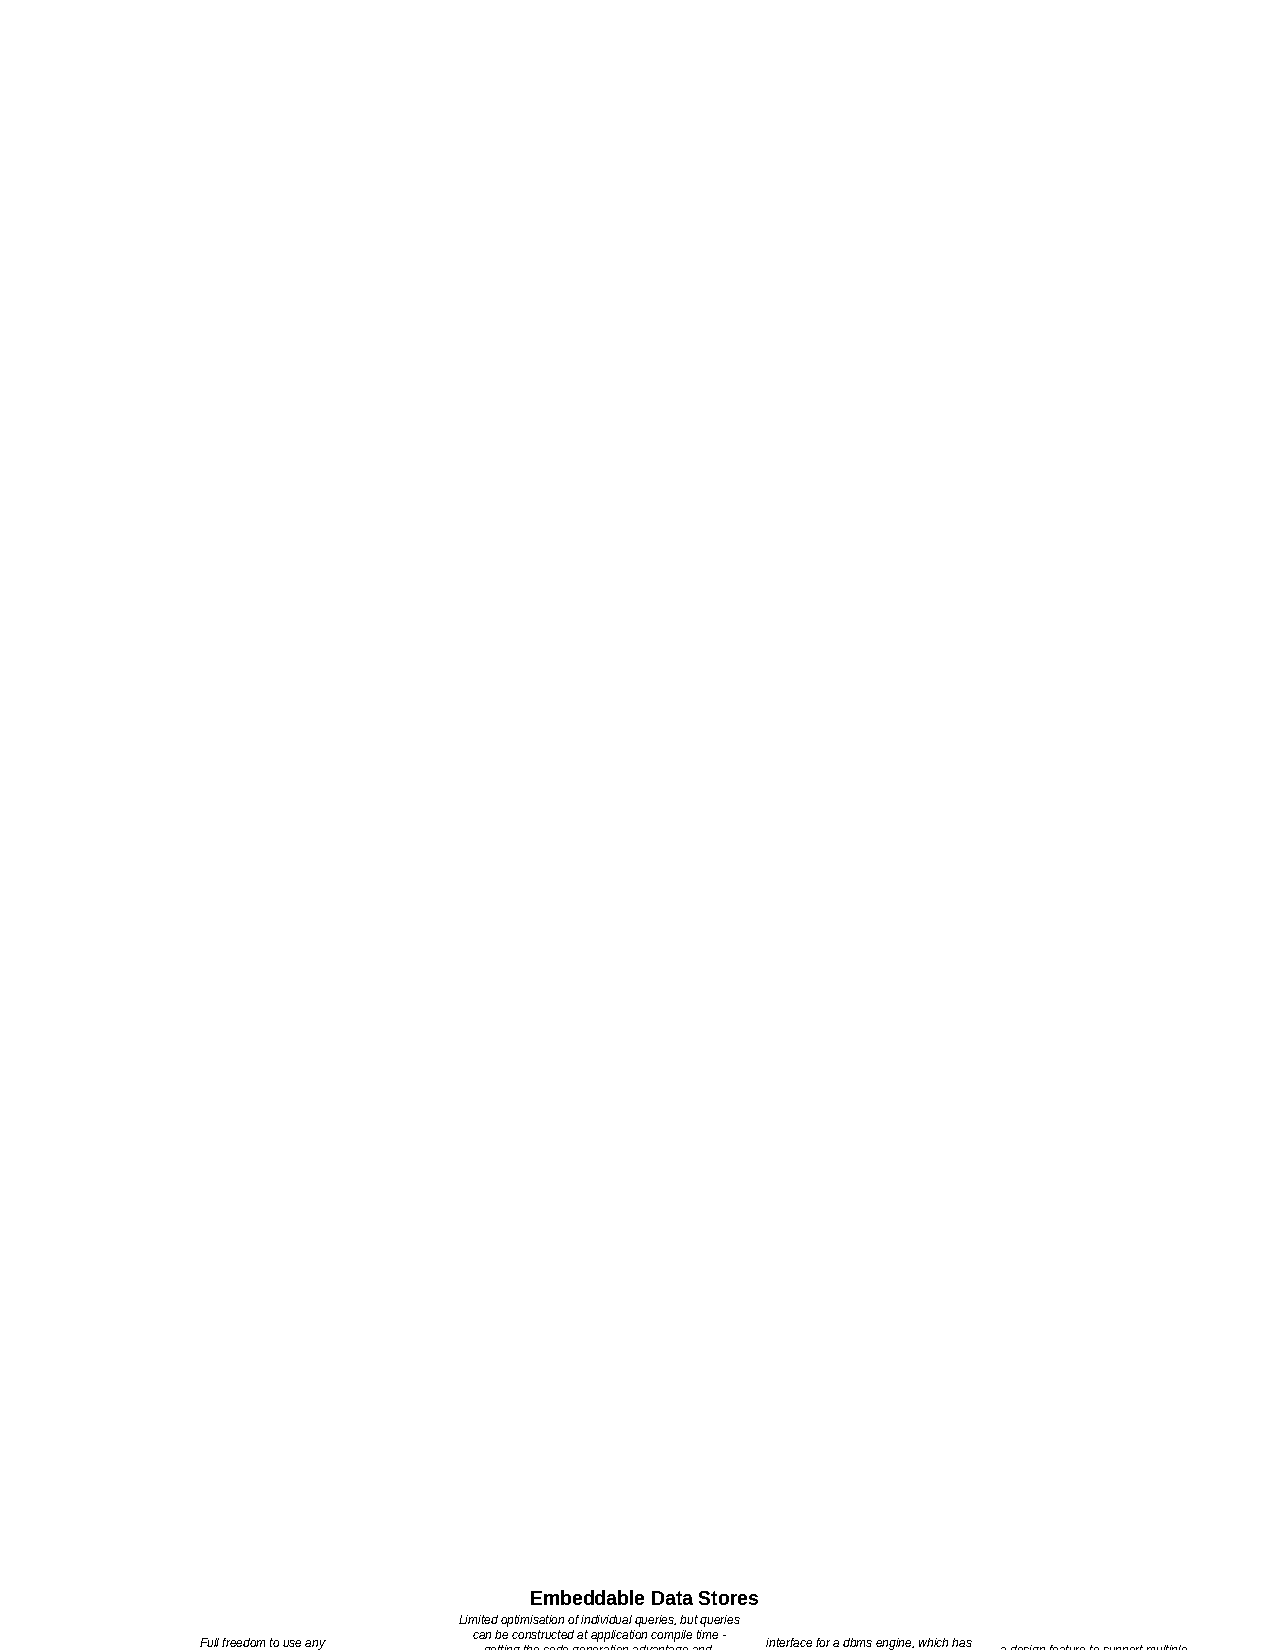
\includegraphics[width=\textwidth]{_drawio/introduction/images/problem_space.pdf}
\end{center}
Unfortunately the strongest abstractions are present in embedded databases that do not take advantage of \ref{lab:known_queries_item} as by design
they both support shcema changes, and are independent from the host language. For example duckDB is embedable in Python, Java, Julia (and other)
applications. The typical embedded database design is just an in-memory database, packaged to be in the same processa an application.
\begin{center}
    \includegraphics[width=\textwidth]{_drawio/introduction/images/typical_system.pdf}
\end{center}
\noindent An ideal system would allow such a datastore to be expressed in a query language, with an embeddable
implementation generated for use, and optimised using the full knowledge of the query set \& schema. It would also provide a strong compile time guarentee on the correctness of all queries.
\begin{center}
    
\includegraphics[width=\textwidth]{_drawio/introduction/images/ideal_system.pdf}
\end{center}
\noindent
No such ideal system exists.
\section{Experimentation}
We can quantify the potential upside of such an ideal system by comparing its performance against both a naive/unoptimised implementation, and against existing embedded databases.
in-memory embedded databases against a \textit{naive} and \textit{foresight} implementations written in rust.
\begin{center}
    \begin{tabular}{l p{.8\textwidth}}
        \textbf{Naive}     & Implemented assuming the provided queries are only a subset of all required. uses a generational arena\cite{TypedGenerationalArenaRepo} that supports insert, delete \& update . \\
        \textbf{Foresight} & Implemented assuming provided queries are the only queries required (as is the case for emdb).                                                                                   \\
    \end{tabular}
\end{center}
\noindent
The schema chosen is designed as a simple OLTP workload, that is too complex to be expressed with a key-value store or dataframes without comparable programmer effort to a manual implementation, by requiring:
\begin{itemize}
    \setlength\itemsep{0em}
    \item Automatically generated unique ids.
    \item Predicate constraints.
    \item Queries that mutate multiple rows in atomic transactions.
    \item Updates collecting returning values.
\end{itemize}
The schema is implemented in the emQL language designed for this project.
\begin{minted}{rust}
table users {
    name: String,
    premium: bool,
    credits: i32,
} @ [ genpk(id), pred(premium || credits > 0) as prem_credits ]
\end{minted}
Both sqlite and duckdb support \mintinline{SQL}{CHECK} constraints for \mintinline{rust}{prem_credits},
in sqlite an \mintinline{SQL}{AUTOINCREMENT} constraint is used for id. In DuckDB a default value
attached to a sequence is used to increment for every insert.
\\
\\ For the naive and foresight implementations we must ensure all writes are checked in advance to ensure the constraint is maintained, or the entire query has no effect.
When multiple rows are changed, this includes iterating through and pre-generating results before applying any.
\begin{minted}{rust}
query new_user(username: String, prem: bool) {
    row(name: String = username, premium: bool = prem, credits: i32 = 0 ) |> insert(users) ~> return;
}
\end{minted}
For the integrated implementations the cost can be reduced to a inserting to an arena, the \mintinline{rust}{username}
does not need to be copied. This demonstrates the advantage in integration, the database implementation can both use the rust string representation (no copy),
and rely on the rust compiler to ensure the string is not mutated from elsewhere.
\\
\\ For the \textit{Foresight} implementation there is an additional early
check on \mintinline{rust}{premium} to place those users in a separate arena, to improve the performance
of the \mintinline{rust}{reward_premium} query that iterate over only premium users.
\\
\\ DuckDB and SQLite both suffer in performance due to the need to construct and then parse the query,
retrieve the cached prepared query, and execute. As a columnar storage DuckDB is at a significant
disadvantage. Performance can be significantly improved by batching the inserts, however this is not possible for many OLTP applications.
\\
\\ This can be seen in the comparative performance.
\begin{center}
    \includegraphics[width=\textwidth]{_plots/introduction/plots/random_insert_boxplot.pdf}
\end{center}

\begin{minted}{rust}
query get_info(user_id: usize) {
    use users |> unique(use user_id as id) ~> return;
}
\end{minted}
For the \textit{foresight} implementation, unlike the others, no copy of the name is required to return the user's information, as no queries mutate the username a reference (qualified to the lifetime of the database) can be used.
\begin{center}
    \includegraphics[width=\textwidth]{_plots/introduction/plots/random_get_ids.pdf}
\end{center}
Note that we do not compare duckDB, it is designed for OLAP and as such it is not does not support fast primary key lookups that determine the time required for these queries.

\begin{minted}{rust}
query get_snapshot() {
    use users |> collect() ~> return;
}
\end{minted}
Much like the \mintinline{rust}{get_info} query, we can use information that no queries ever mutate the username in order to remove the cost of copying strings and instead return a reference qualified to the lifetime of the database.
For this benchmark all names were a simple \mintinline{rust}{"User{id}"} string.
\\
\\ The advantage of the foresight implementation can be arbitrarily increased by making the strings longer \& more expensive to copy.
\begin{center}
    \includegraphics[width=\textwidth]{_plots/introduction/plots/snapshot.pdf}
\end{center}

\begin{minted}{rust}
query add_credits(user: usize, creds: i32) {
    ref users |> unique(use user as id) ~> update(it use credits = credits + creds);
}
\end{minted}
This query is useful only in ensuring it is not possible to optimise the \mintinline{rust}{credits} column away as dead code.
\begin{minted}{rust}
query reward_premium(cred_bonus: f32) {
    ref users
        |> filter(it.premium)
        |> map(user: users::Ref = it, new_creds: i32 = ((it.credits as f32) * cred_bonus) as i32)
        |> update(it use credits = new_creds)
        |> map(creds: i32 = new_creds)
        |> fold((sum: i64 = 0) => (sum = sum + creds))
        ~> return;
}
\end{minted}
The \mintinline{rust}{filter(..)} can be pushed into the \mintinline{rust}{users} relation itself for the \textit{foresight} implementation.
\begin{center}
    \includegraphics[width=\textwidth]{_drawio/introduction/images/reward_loop.pdf}
\end{center}
This is reflected in the benchmarks for both \mintinline{rust}{reward_premium(..)}, and the lower \textit{foresight} performance for \mintinline{rust}{new_user(..)}.
\begin{center}
    \includegraphics[width=\textwidth]{_plots/introduction/plots/reward_premium_users.pdf}
\end{center}
\begin{minted}{rust}
query total_premium_credits() {
    use users
        |> filter(premium)
        |> map(credits: i64 = credits)
        |> fold((sum: i64 = 0) => (sum = sum + credits))
        ~> return;
}    
\end{minted}
We can also keep a view of this query. By updating a counter on changes to the
credits of premium users (at the cost of insert and update) we reduce the query
to a single pointer lookup of a stack value. This can be inlined to remove the
cost of the query function call.
\\
\\ The result is a significant performance improvement, at the cost of updating counters on \mintinline{rust}{new_user(..)}, \mintinline{rust}{add_credits(..)} and \mintinline{rust}{reward_premium(..)}.
\begin{center}
    \includegraphics[width=\textwidth]{_plots/introduction/plots/get_total_prem_credits.pdf}
\end{center}

\section{Objectives}
The objective of the project is to build the following system.
\begin{center}
    \includegraphics[width=\textwidth]{_drawio/introduction/images/emdbprototype.pdf}
\end{center}
This can be broken down into several sub objectives.
\\
\\
\begin{tabular}{l p{.8\textwidth}}
    \textbf{Objective 1.} & \textit{Construct a basic emQL query compiler the supporting a subset of SQL functionality}
\end{tabular}
\begin{quote}
    This will demonstrate the viability of the concept even without complex
    optimisation by allowing seamless embedding of schemas in rust code, and rust code inside schemas.
\end{quote}
\begin{tabular}{l p{.8\textwidth}}
    \textbf{Objective 2.} & \textit{Develop a logical optimiser that demonstrates a performance improvement by using the queries to make data structure choices}
\end{tabular}
\begin{quote}
    None of the currently available systems can take advantage of knowing the entire
    query set, doing so provides a unique optimisation advantage.
\end{quote}
\begin{tabular}{l p{.8\textwidth}}
    \textbf{Objective 3.} & \textit{Implement a comprehensive set of tested, benchmarked example schemas}
\end{tabular}
\begin{quote}
    Important to ensure the correctness of the system, as well as to demonstrate a performance
    improvement by the optimizer over a large variety of plans.
\end{quote}